At the beginning of our project, we tried to automate the whole pipeline in an \emph{end-to-end} deep learning approach starting from the textual input to the generated face. The pipeline is shown in figure \ref{fig:old}.

\begin{figure}[H]
    \centering
    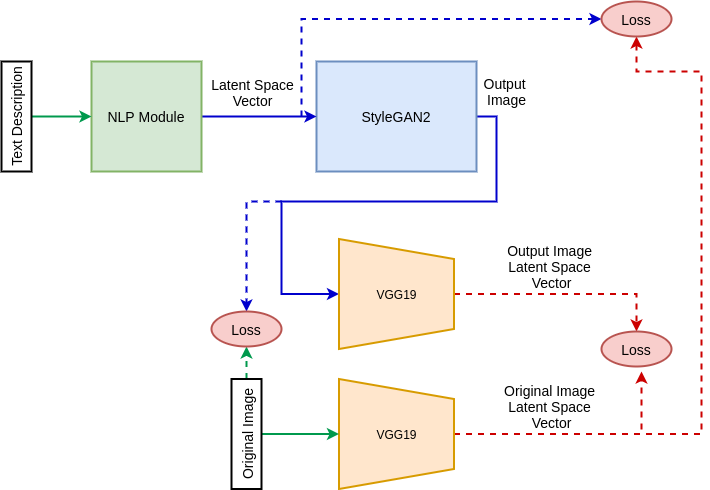
\includegraphics[width=0.7\textwidth]{images/old.png}
    \caption{Old Approach}
    \label{fig:old}
\end{figure}

\subsubsection{Face Generator Module}

We used the same latent-based generative model, which is \texttt{StyleGAN2} with no modifications. We aimed to use the generator pretrained weights to start the \emph{end-to-end} training process, which tunes the generator weights along with the whole system.

\subsubsection{NLP Module}

This module translates the text directly to the \texttt{StyleGAN2} latent vector $z$ that encodes all described facial features. We used a simple \emph{Recurrent Neural Network} (RNN) architecture that consists of $2$ recurrent layers followed by a fully connected layer. This is trained on a semi-synthesized dataset of text, latent vector and face image triplets.

\subsubsection{Dataset and Training}

Our dataset generation and the training process goes as follows :

\begin{itemize}
\item We started by using \emph{Face2Text} dataset that consists of $4000$ records of textual descriptions of images in the \emph{CelebA} dataset.
\item This dataset is very small, so we needed to make it larger :
\begin{itemize}
    \item We used \texttt{FaceNet} \cite{Schroff_2015} to encode the whole \emph{CelebA} dataset, as \texttt{FaceNet} is one of the best facial features extractors.
    \item We used \emph{K-Nearest Neighbors} (KNN) to get the closest $10$ matches of each celebrity in \emph{Face2Text} dataset from \emph{CelebA} dataset.
    \item Then, we manually picked the best $5$ matching faces out of the $10$ faces got from KNN. Therefore, we have a dataset of $20,000$ text-face pairs.
    \item We separately trained a strong feature extractor (\texttt{VGG19}) to map from face images to latent vector, which we called \emph{image-to-latent projector}.
    \item Finally, we used the image-to-latent projector to generate the latent vector corresponding to the dataset faces.
    \item Thus, we had the final dataset triplets of text, latent vector and face image.
\end{itemize}
\item Consequently, we trained our architecture \ref{fig:old} in an \emph{end-to-end} manner using the generated dataset. Mainly, we trained our NLP module and tuned \texttt{StyleGAN2} using a combined loss that consists of the summation of $3$ parts :
\begin{enumerate}
    \item Mean squared error (\emph{MSE}) loss between the output latent vector from NLP module and the project latent vector from the original image.
    \item Reconstruction loss between the output image from \texttt{StyleGAN2} generator using the output latent vector and the original image.
    \item Mean squared error (\emph{MSE}) loss between the projected latent vector of \texttt{StyleGAN2} generator output and the projected latent vector of the original image. This acts as a \emph{perceptual loss} and it's the most important part of our combined loss, as it ensures \emph{cycle consistency}.
\end{enumerate}
\end{itemize}

\subsubsection{Results}

Unfortunately, the previous architecture did not yield good results, due to many reasons :
\begin{itemize}
    \item The dataset was not robust and various enough to train such a huge network.
    \item We did not have enough computational resources to correctly and efficiently train this network for a long time.
    \item The latent space $z$ of \texttt{StyleGAN2} is very sensitive, so the NLP module has to be much more complex to be able to handle the latent vector generation. This was unfeasible given our resources.
\end{itemize}

Consequently, we opt to re-design our system in the staged manner, mentioned above, so that most of the system modules can use unsupervised learning or even no learning at all. 
